\subsection{Microcontroller}

\subsubsection{ESP8266}

\begin{wrapfigure}{r}{0.45\textwidth}
    \vspace{-\baselineskip}
	\centering
	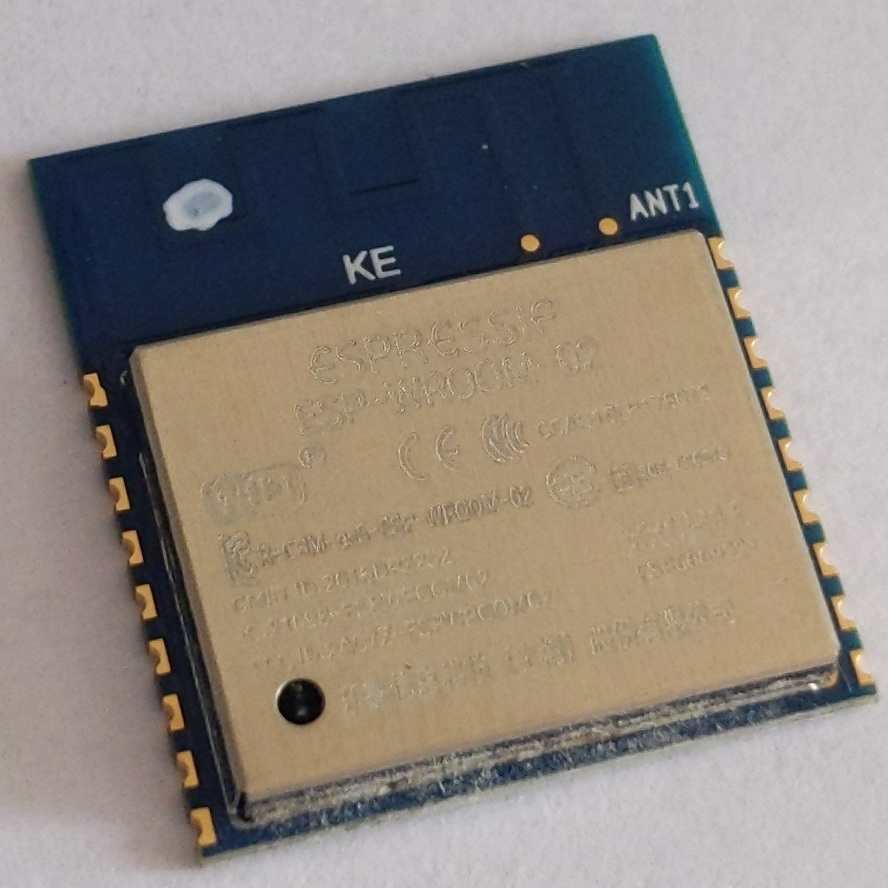
\includegraphics[scale=0.6]{Pictures/esp.jpg}
	\caption{\textit{ESP8266 WROOM-02}}
	\label{img:ESP8266 WROOM-02}
\end{wrapfigure}

Der ESP8266 ist ein 32-Bit \ac{uC} mit einem Systemtakt von 80 - 160MHz. Er verfügt über 64kB \acs{RAM}\label{acro:RAM}, welcher als Arbeitsspeicher genutzt
wird, sowie über 96kB \acs{RAM}, welcher als Datenspeicher genutzt wird. Während des Bootvorgangs wird die Firmware aus einem externen Flashspeicher
geladen. Der \ac{uC} verfügt über alle gängigen Peripherieeinheiten (\acs{ADC},\acs{UART},\acs{SPI},\acs{I2C}\label{acro:SPI}) sowie über eine \acs{WLAN}-Schnittstelle,
welche mit dem Standard \textit{802.11 b/g/n} arbeitet und im 2.4-2,5GHz Band kommuniziert \citep{ESP8266_Datasheet}.

\smallskip

In diesem Anwendungsfall wird der ESP8266 als Modul eingesetzt (ESP8266-WROOM-02), da diese über die nötige externe Beschaltung (Oszillator, Flashspeicher, Antenne)
verfügt \citep{ESP8266_Datasheet}.

\smallskip

Die Programmierung erfolgt über \acs{UART} mittels eines USB-Adapters.

\subsubsection{STM32F103}

Der STM32F103 \ac{uC} basiert auf der Cortex M3 Architektur von ARM und arbeitet mit einem Systemtakt von bis zu 72MHz. Die hier eingesetzte 
Version STM32F103C8 verfügt über 64kB Flashspeicher sowie 20kB \acs{RAM} \citep{STM32_Datasheet}.

\begin{wrapfigure}{r}{0.45\textwidth}
    % \begin{figure}[h]
     \vspace{-\baselineskip}
         \centering
         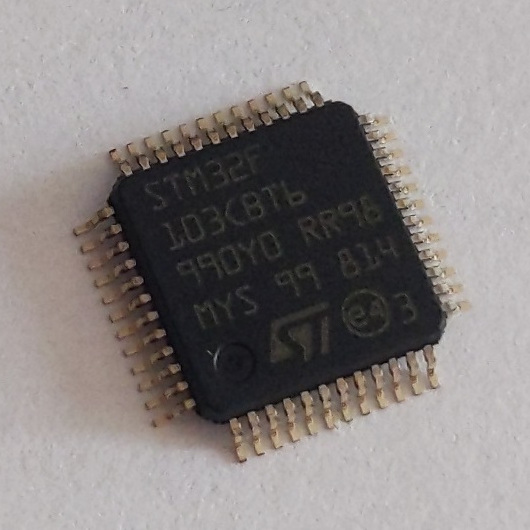
\includegraphics[scale=0.8]{Pictures/stm32f103.jpg}
         \caption{\textit{STM32F103C8}}
         \label{img:STM32F103C8}
    % \end{figure}
 \end{wrapfigure}

\smallskip

An den 37 Ein- und Ausgängen des \acp{uC} sind diverse Kommunikationsschnittstellen verfügbar (\acs{CAN}\label{acro:CAN},\acs{I2C}\label{acro:I2C},\acs{SPI},\acs{USART},\acs{USB}\label{acro:USB}). 
Des Weiteren verfügt der STM32F103 über einen 10-kanaligen 12-Bit \acs{ADC}, diverse Timer mit verschiedenem Funktionsumfang
sowie über einen \acs{DMA}-Controller \citep{STM32_Datasheet}. 

\smallskip

Für die Programmierung des \ac{uC} ist ein ST-Link Programmiergerät notwendig, welches auch Debugging ermöglicht \citep{STM32_Datasheet}.


